\section{Plasticine Specialization for RNN Serving} \label{sec:rnn_arch}

Low-precision inference are commonly used to reduce memory footprint of deep learning models and
increase compute density of hardware accelerators.
Plasticine, however, only supports 32-bit operations and datapath.
Using RNN serving as a motivating example, this section discusses the necessary architecture augmentation and
specialization needed to efficiently map real-time inference on Plasticine.

Recurrent Neural Networks (RNNs) are a class of sequence models that plays a key role
in low-latency, AI-powered services in datacenters \cite{fowers2018configurable, jouppi2017datacenter}.
These applications have stringent tail latency requirements, within the window of miliseconds,
for real-time human computer interactions.
An example of such workload is
Google Translate; inference runs concurrently as the user types.
An efficient acceleration of RNN requires flexible datapath to support global optimizations beyond
BLAS kernels, which is where dataflow accelerators like Plasticine would shine.
To meet this low-latency requirement, the other prerequisite is that everything has to stay on-chip.
To achieve this, we introduce a limited mixed-precision support with changes localized to PCUs. 
The enhancement supports the commonly used precision in machine learning without introducing massive
overhead from fine-grained reconfigurability.

In the remaining of this secction, \Cref{sec:lowprec} proposes the necessary micro-architectural changes to
  support low-precision arithmetics on Plasticine.
\Cref{sec:foldrt} introduces a folded reduction structure in PCU's SIMD that improves the function
unit (FU) utilization.
\Cref{sec:sizing} discusses architectural parameter selection for Plasticine
  to serve RNN applications efficiently.

\subsection{Mixed-Precision Support} \label{sec:lowprec}
\label{sec:arch:varprec}
Previous works \cite{fowers2018configurable, jouppi2017datacenter}
  have shown that low-precision inference can deliver promising performance
  improvements without sacrificing accuracy.
In the context of reconfigurable architectures such as FPGAs,
  low-precision inference not only increases compute density,
  but also reduces required on-chip capacity for
  storing weights and intermediate data.

To support low-precision arithmetics without sacrificing coarse-grained reconfigurability,
we introduce two low-precision struct types in Spatial: a tuple of 4 8-bit and 2 16-bit floating-point 
numbers, \texttt{4-float8} and \texttt{2-float16} respectively.
Both types packs multiple low-precision values into a single precision storage.
We support only 8 and 16-bit precisions, which are commonly seen in deep learning inference hardwares.
Users can only access values that are 32-bit aligned.
This constraint guarantees that the microarchitectual change is only local to the PCU.
PMU and DRAM access granularity remains intact from the original design.

\begin{figure}
  \centering
  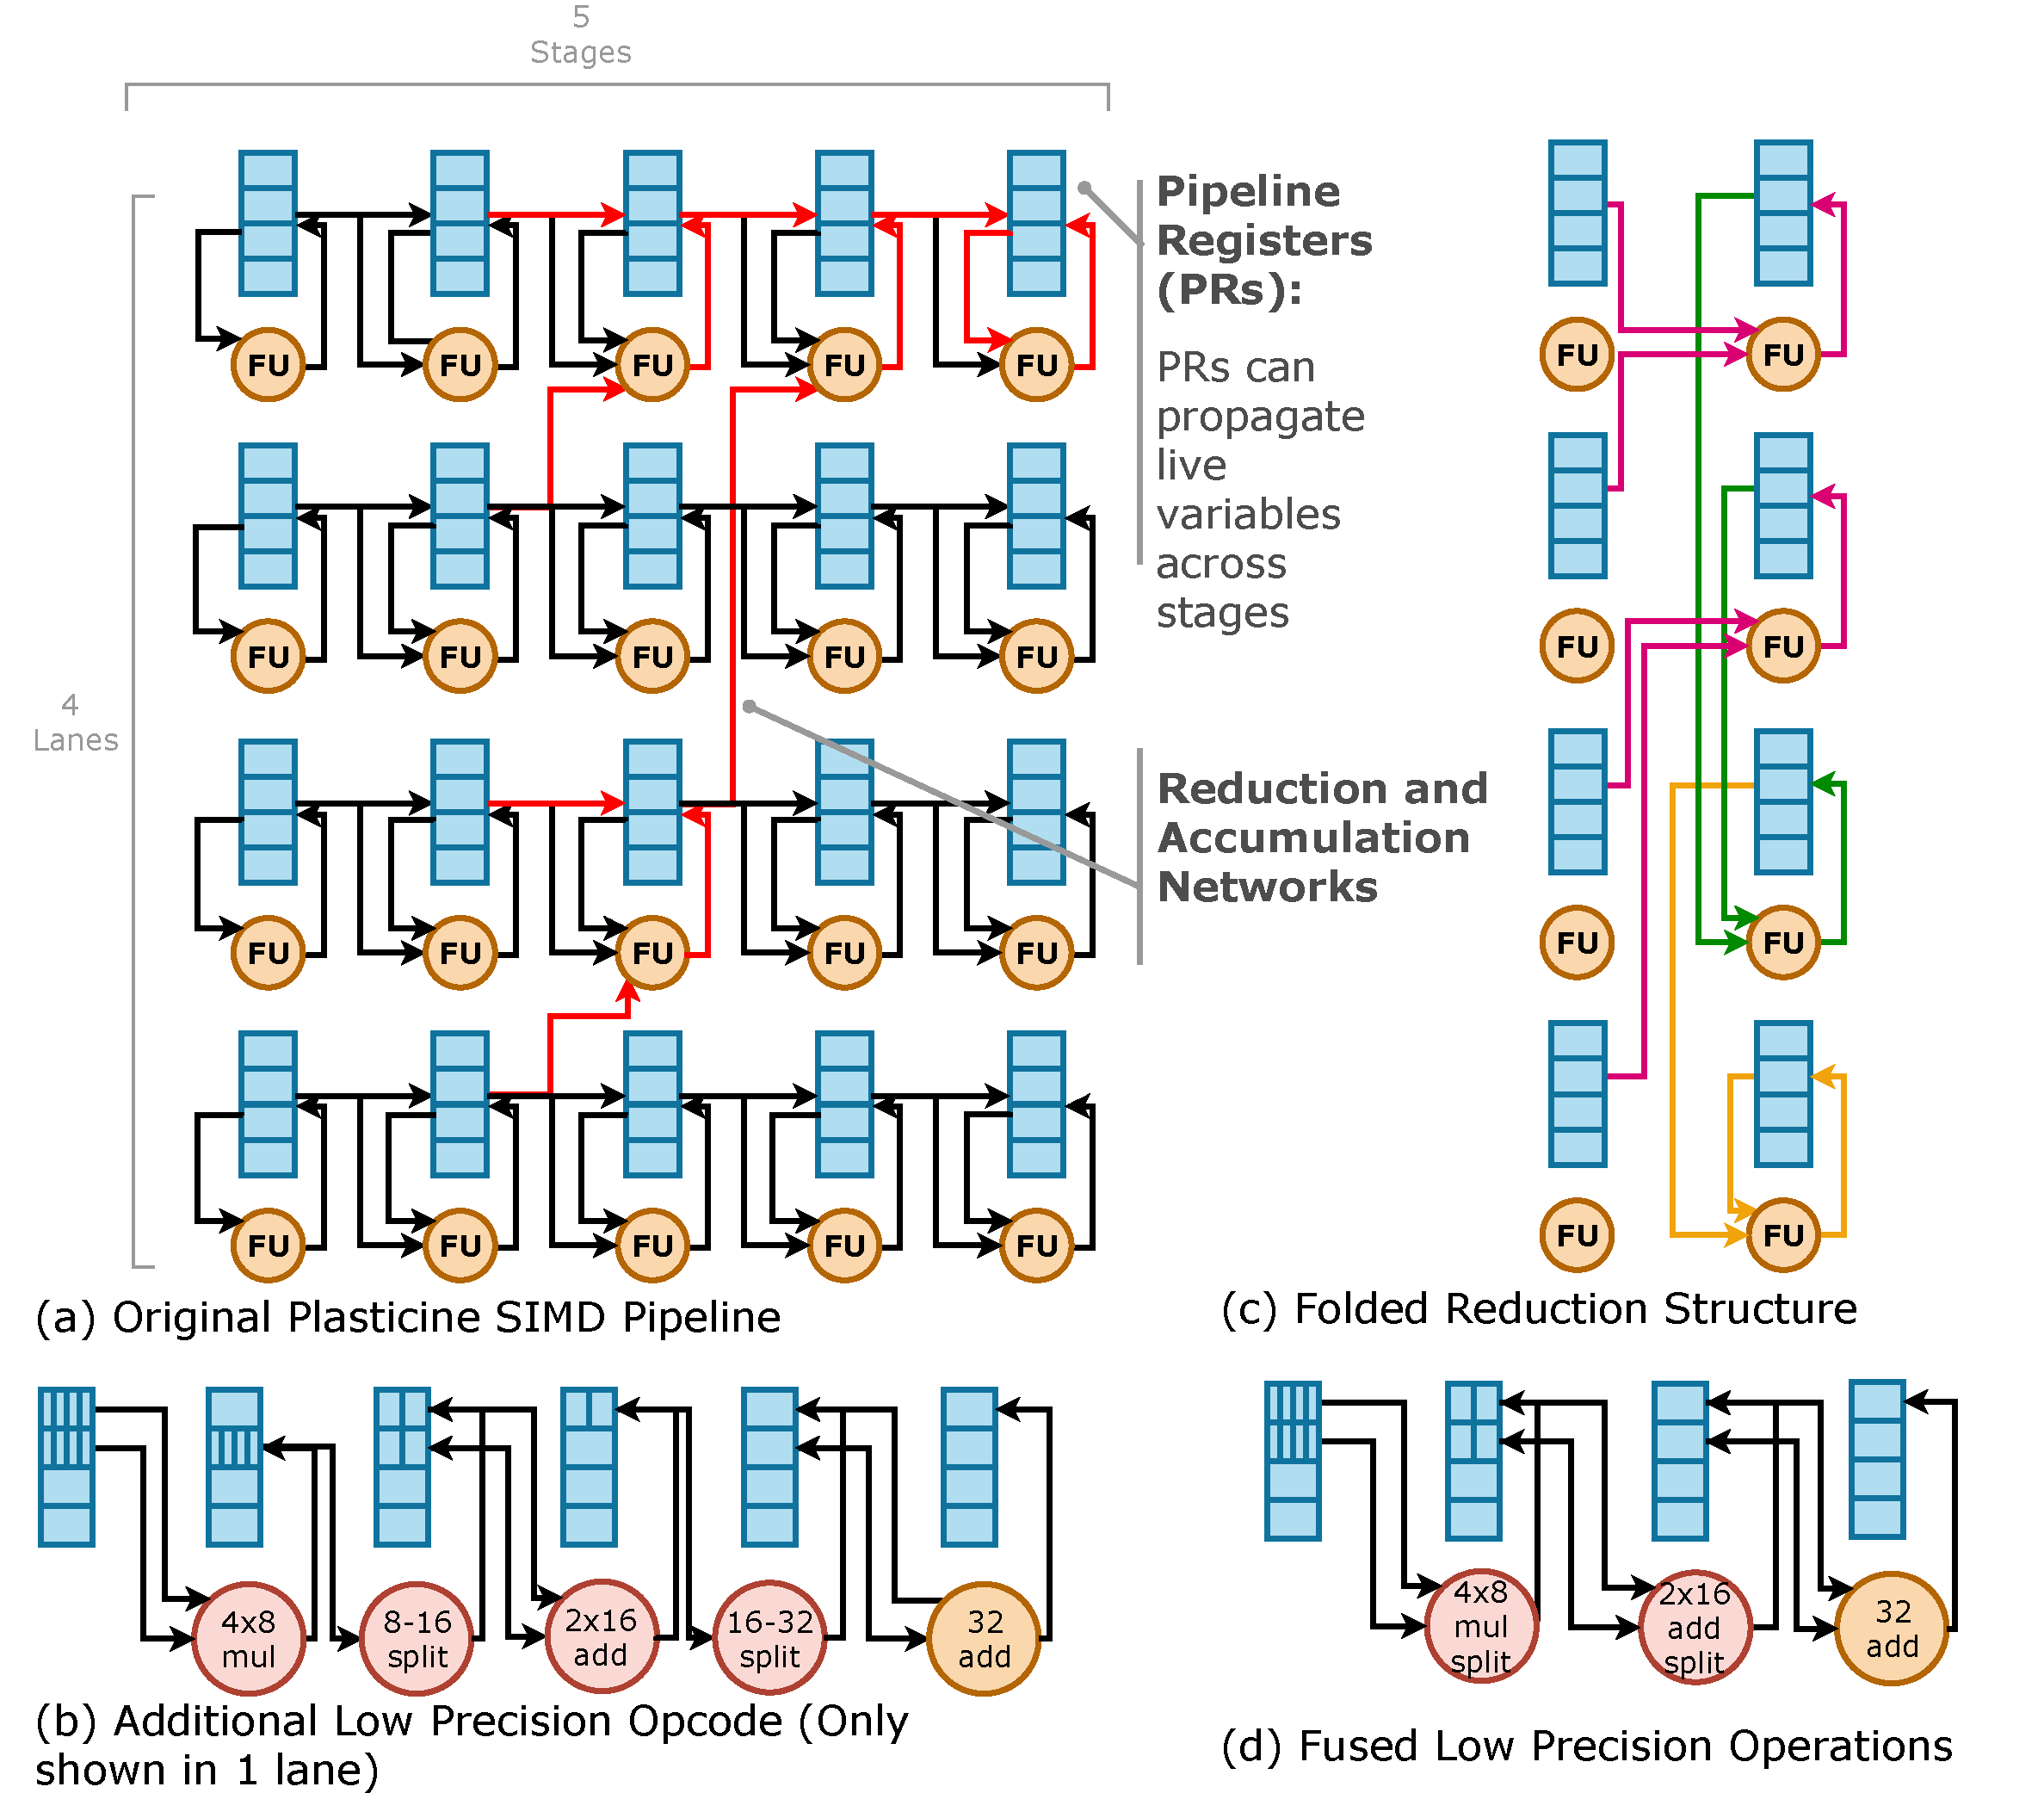
\includegraphics[width=1\columnwidth]{figs/lowprec.pdf}
  \caption{Plasticine PCU SIMD pipeline and low-precision support.
  Red circles are the new operations. Yellow circles are the original opertaions in Plasticine.
  In (d) the first stage is fused $1^{st}, 2^{nd}$ stages, and the second stage is fused
  $3^{nd}$, $4^{th}$ stages of (b).
   }
  \label{fig:lowprec}
\end{figure}
Figure \ref{fig:lowprec} (a) shows the original SIMD pipeline in a Plasticine PCU.
Each FU supports both floating-point and fix-point operations.
When mapping applications on Plasticine,
  the inner most loop body is vectorized across the lanes of the
SIMD pipeline, and different operations of the loop body are mapped to different stages.
Each pipeline stage contains a few pipeline registers (PRs)
  that allow propagation of live variables across stages.
%The PRs are accessible as both inputs and outputs of the FU.
%An FU can also read previous stage's PRs
%as its input value.
Special cross-lane connections as shown in red in Figure \ref{fig:lowprec} enable reduction operations.
To support 8-bit element-wise multiplication and 16-bit reduction, we add 4 opcodes to the FU, shown in
Figure \ref{fig:lowprec} (b).
The $1^{st}$ and $3^{rd}$ stages are element-wise, low-precision operations
  that multiply and add 4 8-bit and 2 16-bit values, respectively.
The $2^{nd}$ and $4^{th}$ stages rearrange low-precision values into two registers,
  and then pad them to higher precisions.
The $5^{th}$ stage reduces the two 32-bit value to a single 32-bit value using the existing add operation. 
From here, we can use the original
reduction network shown in Figure \ref{fig:lowprec} (a) to complete the remaining reduction and accumulates
in 32-bit connection.

With 4 lanes and 5 stages,
  a PCU first reads 16 8-bit values,
  performs 8-bit multiplication followed by rearrangement and padding,
  and then produce 16 16-bit values after the second stage.
The intermediate values are stored in 2 PRs per lane.
Next, 16 16-bit values are reduced to 8 16-bit values
  and then rearranged to 8 32-bit value in 2 PRs per lane.
Then, the element-wise addition in 32-bit value
  reduces the two registers in each line into 4 32-bit values.
These values are fed through the
  reduction network that completes the remaining
  reduction and accumulation in two plus one stages.

In a more aggressive specialization,
  we can fuse the multiply and rearange into the same stage.
We also fuse the first low-precision reduction with the next rearange as shown in Figure \ref{fig:lowprec} (d).
In this way, we can perform the entire low-precision map-reduce in 2 stages
  in addition to the original full precision reduction.
In order to maximize hardware reuse,
  we assume that it is possible to construct a full precision FU
  using low-precision FUs.

\subsection{Folded Reduction Tree} \label{sec:foldrt}
The original reduction tree shown in \Cref{fig:lowprec} (a) requires $\log_2(\#_{LANE})+1$ number of
stages for $\#_{LANE}$ operations, leading to a low utilization of the FUs in the SIMD pipeline.
The reduction tree also restricts the SIMD pipeline to have at least 
$\log_2(\#_{LANE})+1$ stages to compute a full reduction within a PCU.
For a SIMD pipeline with 16 lanes, the FU utilization is only 53.33\% in reduction stages.

To improve FU utilization, we introduce a folded reduction structure that performs $\#_{LANE}$
operations entirely within a single stage, pipelined over multiple cycles.
Figure \ref{fig:lowprec} (c) shows the folded reduce-accumulate structure.
Instead of feeding the output of the reduction operation to the next stage, 
this structure folds the output back to the PR of the next unused FU in the 
same stage. 
The entire reduction plus accumulation is still fully pipelined in $\log_2(\#_{LANE})+1$ cycles
with no structural hazard.
In the original design, only a single register among the PRs have the special reduction tree
connection.
The down side of the folded structure is that no other live variables can be propagated after this
reduction stage, unless adding multiple folded trees. 
In applications, we rarely see the need of multiple live variables after the reduction operation
other than the accumulator itself.
Therefore, it makes the most sense to put the
folded reduction tree only in the last stage of a SIMD pipeline.

With the fused reduced-precision operations and the folded reduction tree,
  a PCU is able to perform 64 8-bit map-reduce in 4 stages, and 32 16-bit map-reduce in 3 stages.
All the operations are still completed in $2+\log_2(\#_{LANE})$ cycles, i.e. 
8, 7, and 6 cycles for 8-, 16-, and 32-bit operations, respectively.

\subsection{Sizing Plasticine for RNN Serving} \label{sec:sizing}
Evaluating an RNN cell containing $N$ hidden units and $N$ input features
  requires $2N^2$ computations and $N^2+N$ memory reads.
With large $N$, the compute to memory ratio is 2:1.
The original Plasticine architecture uses a checkerboard layout
  with 1 to 1 ratio between PCU and PMU.
A PCU has 6 stages and 16 lanes, and a PMU has 16 banks.
This provides a 6:1 ratio between
  compute resource and on-chip memory read bandwidth.
As a result of this layout,
  on-chip memory read bandwidth becomes the bottleneck for accelerating RNN serving applications.
Given that RNNs cover a wide range of important applications,
  we select a Plasticine configuration tailored for RNN serving.
Specifically, we choose a 2 to 1 PMU-PCU ratio with 4 stages in each PCU.
Figure \ref{fig:arch} shows the layout of this Plasticine variant.
\begin{figure}
  \centering
  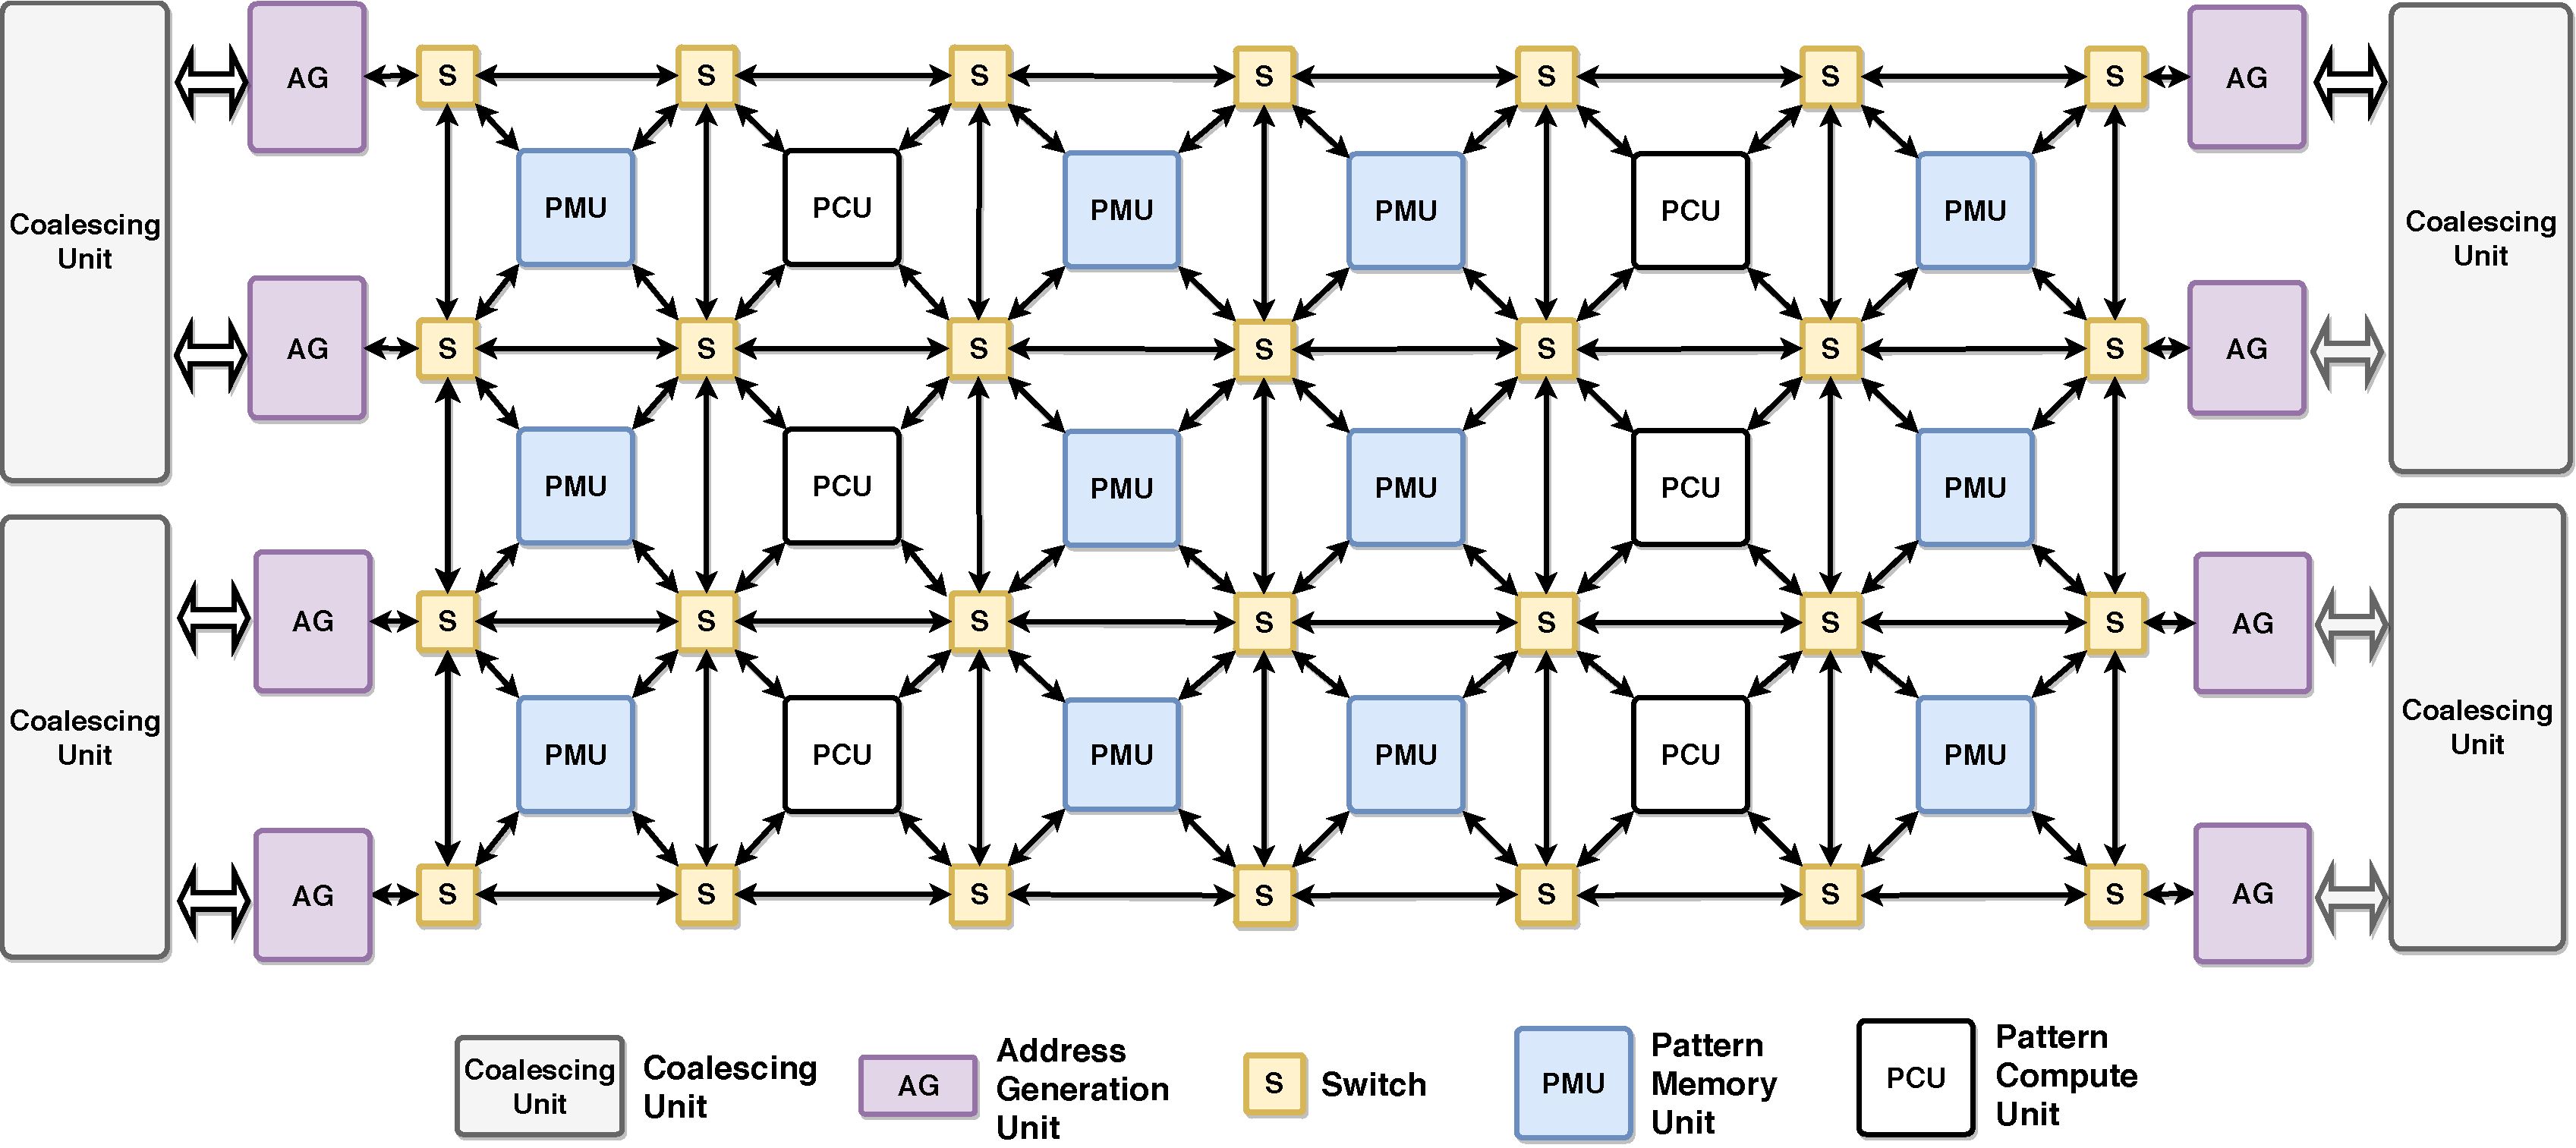
\includegraphics[width=\textwidth]{figs/rnnarch.pdf}
  \caption[Variant Plasticine configuration for RNN serving]{
    Variant Plasticine configuration for RNN serving with 2:1 ratio for PMU and PCU}
  \label{fig:arch}
\end{figure}
